\documentclass[UTF8]{ctexart}
\usepackage{geometry}
\geometry{margin=1.5cm, vmargin={0pt,1cm}}
\setlength{\topmargin}{-1cm}
\setlength{\paperheight}{29.7cm}
\setlength{\textheight}{25.3cm}

% 常用宏包
\usepackage{amsfonts}
\usepackage{amsmath}
\usepackage{amssymb}
\usepackage{amsthm}
\usepackage{enumerate}
\usepackage{graphicx}
\usepackage{multicol}
\usepackage{fancyhdr}
\usepackage{layout}
\usepackage{listings}
\usepackage{float}
\usepackage{caption}
\usepackage{graphicx}

\lstset{
    basicstyle=\ttfamily, 
    basewidth=0.5em
}

% 自定义命令
\newcommand{\dif}{\mathrm{d}}
\newcommand{\avg}[1]{\left\langle #1 \right\rangle}
\newcommand{\difFrac}[2]{\frac{\dif #1}{\dif #2}}
\newcommand{\pdfFrac}[2]{\frac{\partial #1}{\partial #2}}
\newcommand{\OFL}{\mathrm{OFL}}
\newcommand{\UFL}{\mathrm{UFL}}
\newcommand{\fl}{\mathrm{fl}}
\newcommand{\op}{\odot}
\newcommand{\Eabs}{E_{\mathrm{abs}}}
\newcommand{\Erel}{E_{\mathrm{rel}}}

\begin{document}

\pagestyle{fancy}
\fancyhead{}
\lhead{李慧一, 12435055}
\chead{数据结构与算法第四次作业}
\rhead{2024年10月20日}

\section{测试程序的设计思路}

我一共创建了5个链表。

第一步,我通过默认构造函数建立了第一个链表 \texttt{lst}。使用 \texttt{.push\_back()} 和 \texttt{.push\_front()} 分别在尾部和首部插入左值数据,并在两端插入右值数据后输出结果;
进一步使用 \texttt{.pop\_front()} 和 \texttt{.pop\_back()} 分别在首部和尾部删除数据并输出结果,在其中通过for循环测试了\texttt{前置自增运算符++}、\texttt{*操作符}、\texttt{.begin()}、\texttt{end()};
进一步,我分别通过\texttt{++、--}操作获得不同位置的迭代器,输出结果证明了\texttt{前置自减和后置递减--}运算符的正确性;
在之后,我分别通过\texttt{.insert()}将左值数据和右值数据插入在指定位置;
最后,我通过\texttt{.erase()}分别删除了指定位置和指定范围的数据。

第二步,我通过列表初始化构造函数建立了第二个链表\texttt{lst2},在其中验证了后置递增运算符++,并输出结果。

第三步,我通过拷贝构造函数,将链表\texttt{lst2}深度复制给了链表\texttt{lst3},并输出\texttt{lst3}的结果。

第四步,我通过移动构造函数,将链表\texttt{lst3}作为右值构造了链表\texttt{lst4},并输出\texttt{lst4}的结果。

第五步,我首先构造了链表\texttt{lst5},并通过重载的赋值运算符\texttt{=},将\texttt{lst4}复制给\texttt{lst5},在其中实现了深拷贝;
并对\texttt{front()、.back()、begin()、end()}进行了非常量对象的测试,结果显示此时在读取数据后可以进行修改,而若是常量对象,则只有只读权限;
最后,我对于该链表分别进行了\texttt{.size()、.clear()、empty()}测试,结果显示成功实现了清空。

此外,针对析构函数,我在原析构函数的基础上添加了一行输出,结果显示了多次析构函数的调用。



\section{测试的结果}
上述过程的所有结果展示如下,在用 \texttt{valgrind} 进行测试后,未发现内存泄漏。

\begin{figure}[h]
    \centering
    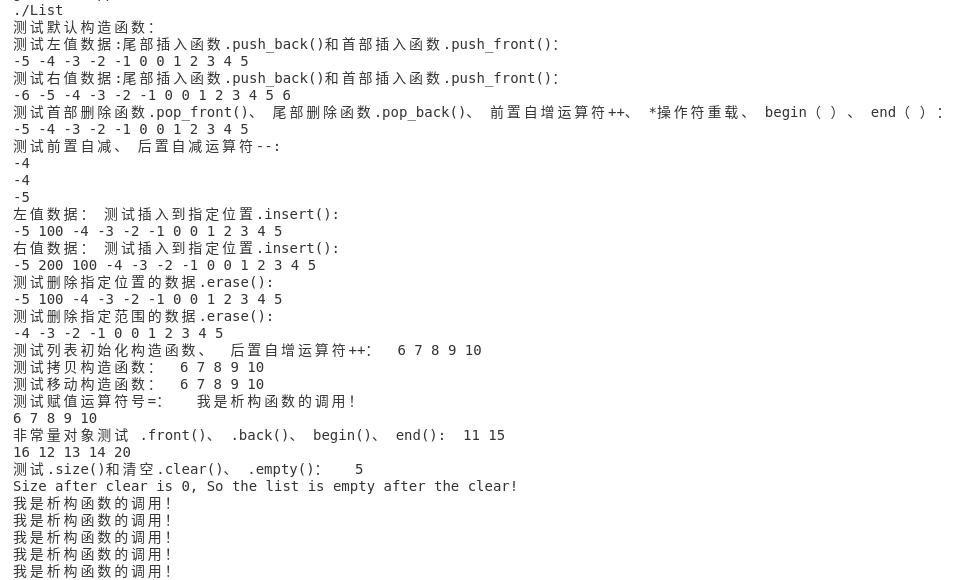
\includegraphics[width=0.85\textwidth]{result.png} % 替换为你的图片文件名
    \caption{Result}

\end{figure}

\begin{figure}[h]
    \centering
    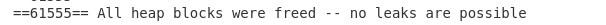
\includegraphics[width=0.75\textwidth]{valgrind.png} % 替换为你的图片文件名
    \caption{Valgrind}
\end{figure}

\end{document}
